\section*{Introduction to Vehicle Dynamics}

\begin{frame}{What is Vehicle Dynamics?}
    \begin{columns}
        \column{0.6\textwidth}
        Vehicle Dynamics is the study of how a vehicle moves. \\
        \vspace*{2ex}
        In USM, we are responsible for anything related to performance:
        \begin{itemize}
            \item Laptime simulation
            \item Testing planning and execution
            \item Driver development
            \item Data analysis
            \item Engineering Challenge
            \item Laptime Simulation Event
        \end{itemize}
        \column{0.4\textwidth}
        \begin{figure}
            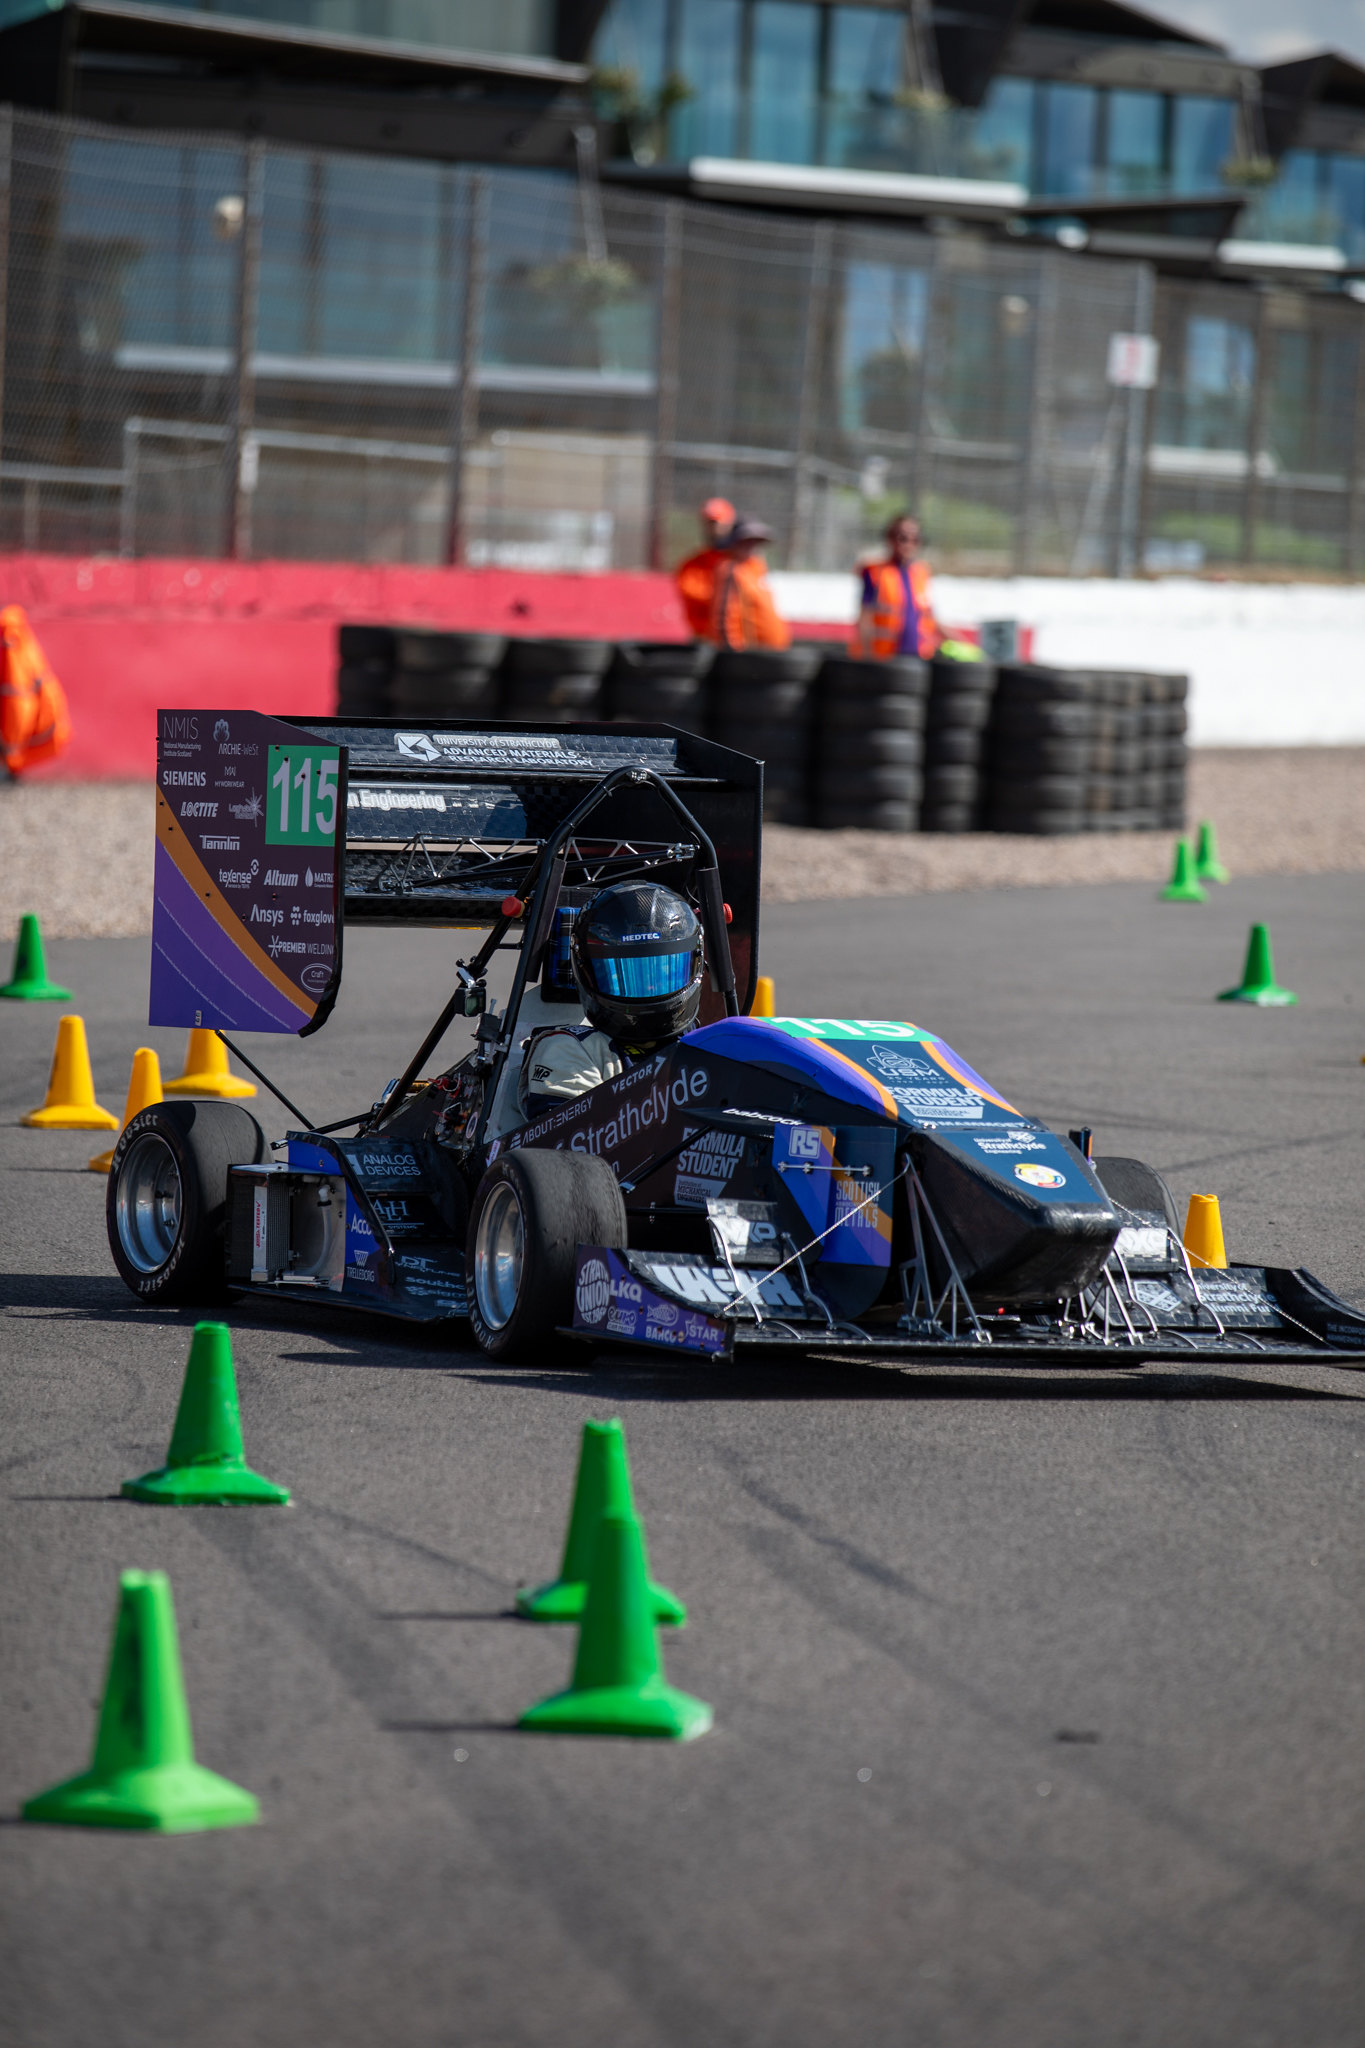
\includegraphics[width=\textwidth]{../../res/car/FSUK Cornering.jpg}
        \end{figure}
    \end{columns}
\end{frame}

\begin{frame}{Semester 1 Teaching Schedule}
    \begin{table}
        \renewcommand{\arraystretch}{1.5}
        \begin{tabular}{l l l}
            \textbf{Week} & \textbf{Date} & \textbf{Topic} \\
            \hline
            Week 2 & 30/09/2025 & System introduction \\
            Week 3 & 06/10/2025 & Velocity-Acceleration plot \\
            Week 4 & 13/10/2025 & GG plot \\
            Week 5 & 20/10/2025 & Introduction to laptime simulation \\
            Week 6 & 27/10/2025 & Load transfer \\
            Week 7 & 03/11/2025 & GGV plot \\
            Week 8 & 10/11/2025 & Tyres \\
            Week 9 & 17/11/2025 & Advanced laptime simulation \\
            Week 10& 24/11/2025 & Advanced tyres

        \end{tabular}
    \end{table}
\end{frame}